%\subsection{Aplicativo}

	\par Para iniciar a construção do aplicativo, fez-se necessário a instalação e
configuração do ambiente de desenvolvimento. Primeiramente, realizou-se o
\textit{download} da IDE Android Studio, versão 1.1.0 e do Android SDK, versão
24.0.2, ambos no site \textit{Developers} Android através do endereço
https://developer.android.com/intl/pt-br/sdk/index.html.

	\par Contudo, ao executar o emulador do Android o sistema apresentava a
seguinte mensagem: \textit{"emulator: Failed to open the HAX device!"}.
Depois de algum tempo pesquisando, percebeu-se que era necessário instalar um programa
chamado \textit{Intel Hardware Accelerated Execution Manager} (HAXM), que
permite a execução emulador Android mais rápido.

	\par No entanto, ao instalá-lo ocorria o seguinte erro:\textit{ “this computer
meets the requirements for haxm but intel virtualization technology (VT-x) is
not turned on”}.  A solução foi acessar a BIOS da máquina e habilitar o
assistente de hardware para virtualização. Daí em diante, foi possível executar
no emulador as aplicações feitas no Android Studio.

	\par Com o ambiente já configurado, foi criado um repositório no controlador de
versão Github, o qual pode ser acessado através do endereço
https://github.com/diegodnunes12/AppTCC e compartilhado entre os participantes
do projeto.

	\par A partir de então, passou-se a desenvolver o software. A princípio, foi
construída uma \texttt{activity}, que é acessível ao aluno logo que a aplicação
se inicia. Essa \texttt{activity} é do tipo Navigation Drawer Layout, ou seja,
é um painel que permite inserir as opções de navegação do aplicativo,
semelhante a um menu.

	\par Ao criar essa \texttt{activity}, o Android Studio gera automaticamente
a classe \texttt{NavigationDrawerFragment} e um arquivo XML na pasta
\textit{layout}, chamado \texttt{fragment\_navigation\_drawer.xml}.

	\par No arquivo \texttt{fragment\_navigation\_drawer.xml} foram inseridos três
\textit{widgets}, sendo dois do tipo \texttt{textView}, para o cabeçalho com a
logomarca da Univás e para o rodapé com o seguinte texto: “Univás – Pouso
Alegre – MG” e um \textit{widget} do tipo \texttt{listView} que contém a lista
com as opções que o software oferece ao aluno.

	\par O \textit{layout} desta \textit{activity} chama-se o
\texttt{relativeLayout}, o qual permite adicionar um elemento em relação ao
outro. Desta forma o \textit{widget} \texttt{listView} utiliza o comando
\texttt{android:layout\_below="@+id\/headerView} para se posicionar após o
componente com id \textit{headerView} e a instrução
\texttt{android:layout\_above="@+id\/footerView"} indicando que ela deve
preceder o \textit{widget} com id \textit{footerView}. Na Figura \ref{fig:app},
pode ser visto o código XML dos \textit{widgets} desta tela.

	\begin{figure}[h!] 
		\centerline{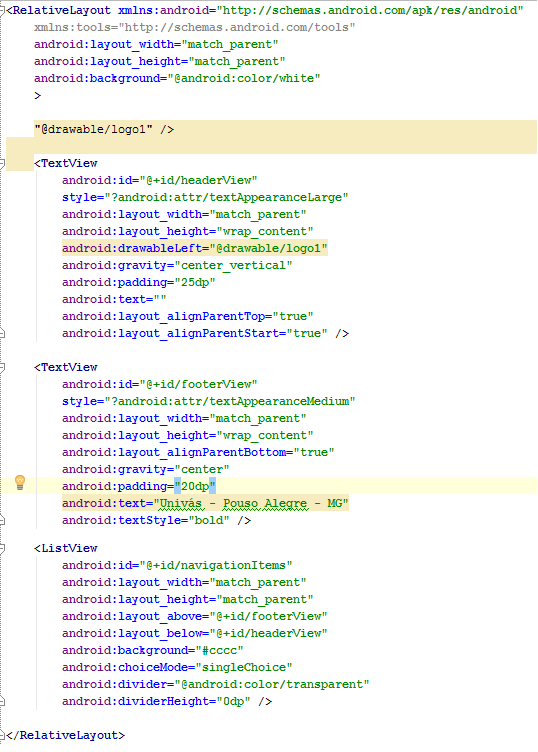
\includegraphics[scale=0.8]{./imagens/2_q_metodologico/4_procedimentos_resultados/42_aplicativo/app.png}}
		\caption[Código XML dos widgets do arquivo
		fragment\_navigation\_drawer.xml]{Código XML dos widgets do arquivo
		\texttt{fragment\_navigation\_drawer.xml}.
		\textbf{Fonte:}Elaborado pelos autores.}
		\label{fig:app}
	\end{figure}
	
	\pagebreak

	\par A classe \texttt{NavigationDrawerFragment} representa o painel de
navegação. Nela se destaca o método \texttt{onCreateView()}, responsável por
criar o \textit{layout} de navegação. Na Figura \ref{fig:app1}, vê-se o método
\texttt{onCreateView()} informando ao sistema operacional o \texttt{layout} a
ser chamado e adicionando a um \textit{array} de \textit{String} as
alternativas de navegação que serão exibidos no \textit{listView} da tela
principal.

	\begin{figure}[h!] 
		\centerline{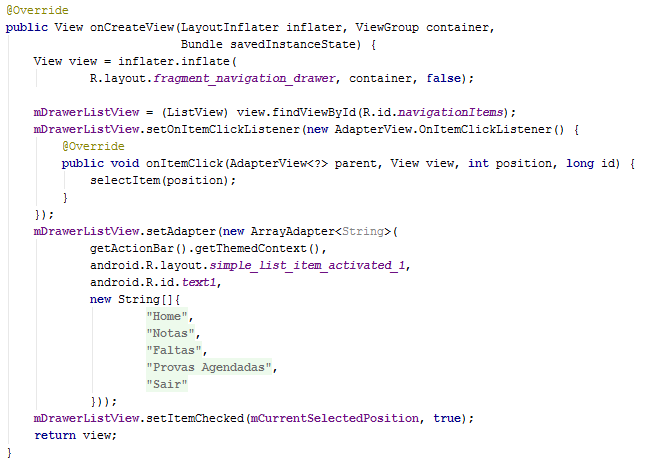
\includegraphics[scale=0.7]{./imagens/2_q_metodologico/4_procedimentos_resultados/42_aplicativo/app1.png}}
		\caption[Método onCreateView()]{Método \texttt{onCreateView()}.
		\textbf{Fonte:}Elaborado pelos autores.}
		\label{fig:app1}
	\end{figure}
	
	\pagebreak
	
	\par O próximo passo foi criar o banco de dados do aplicativo para salvar as
informações recebidas do \textit{web service}. Para que isso fosse possível,
elaborou-se uma classe denominada \texttt{DatabaseHelper} que estende da classe
\texttt{SQLiteOpenHelper} do Android, com dois métodos, um chamado
\texttt{onCreate()} que cria a estrutura do banco de dados e outro conhecido
por \texttt{onUpgrade()}, usado se for necessário atualizar a estrutura do
banco de dados.

	\par Foi preciso criar um atributo que mantém a versão do banco de dados. Essa
informação serve para que o Android consiga saber qual dos dois métodos devem
ser executados. Ao iniciar a aplicação pela primeira vez, estando a versão em 1
(um), o sistema chamará o método \texttt{onCreate()}. Se for preciso atualizar
a estrutura do banco, o atributo versão deve ser incrementado em 1 (um), de
modo que ao executar o software o sistema operacional perceba a mudança,
chamando o método \texttt{onUpgrade()}. Na Figura \ref{fig:app2} é apresentado a
classe \texttt{DatabaseHelper}.

	\begin{figure}[h!] 
		\centerline{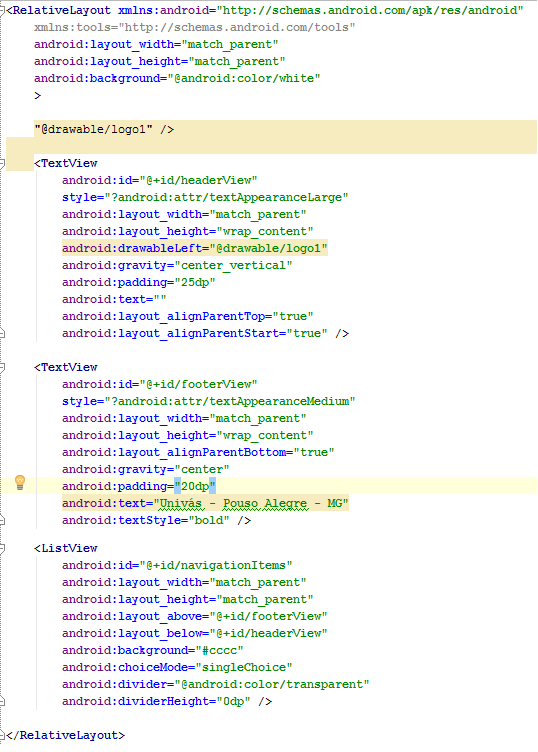
\includegraphics[scale=0.7]{./imagens/2_q_metodologico/4_procedimentos_resultados/42_aplicativo/app2.png}}
		\caption[Classe DatabaseHelper]{Classe \texttt{DatabaseHelper}.
		\textbf{Fonte:}Elaborado pelos autores.}
		\label{fig:app2}
	\end{figure}
	
	\pagebreak
	
	\par Em seguida foi criada a classe responsável por executar as consultas SQL,
denominada \texttt{DatabaseExecute}. Nela foram inseridos os métodos
responsáveis por inserir, alterar e buscar os dados dos alunos no banco de
dados local do aplicativo. Na Figura \ref{fig:app3}, pode se observar o método
que possibilita a inserção dos eventos ocorridos. Esses eventos podem ser notas,
faltas ou provas agendadas.

	\begin{figure}[h!] 
		\centerline{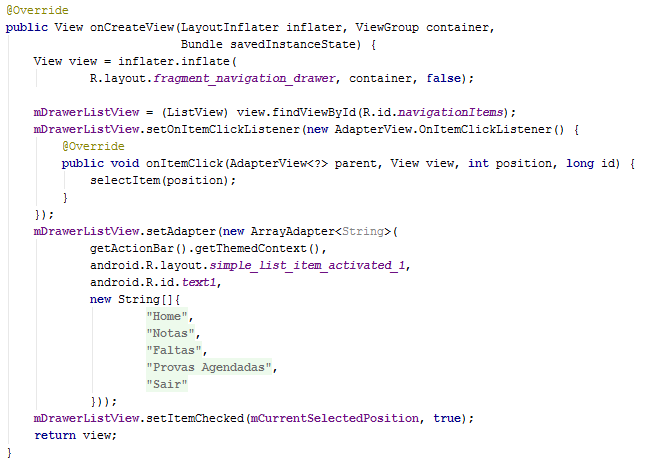
\includegraphics[scale=1]{./imagens/2_q_metodologico/4_procedimentos_resultados/42_aplicativo/app3.png}}
		\caption[Método de inserção de eventos]{Método de inserção de eventos.
		\textbf{Fonte:}Elaborado pelos autores.}
		\label{fig:app3}
	\end{figure}
	
	\pagebreak
	
	\par Este método recebe um objeto da classe \texttt{EventTO} com os elementos
necessários para inserir o evento no banco de dados. Para que seja possível a
inserção dos dados, \citeonline{monteiro2012}, afirma que é necessário
recuperar a referência da classe \texttt{SQLiteDatabase} através do método
\texttt{getWritableDatabase()}, logo após é instanciada a classe
\texttt{ContentValues}, onde é informado o campo da tabela e o valor desejado.
Ao concluir, é chamado o \texttt{insert} da classe \texttt{SQLiteDatabase}
informando o nome da tabela e o objeto da classe \texttt{ContentValues}.

	\par Para listar os resultados dos exames realizados pelos discentes no painel
de notas é utilizado o método \texttt{getResults()} que retorna uma lista de
objetos da classe \texttt{EventTO}. De acordo com \citeonline{monteiro2012},
para conseguir recuperar as informações armazenadas no banco de dados é preciso
adquirir a instância de leitura da classe \texttt{SQLiteDatabase} através do
método \texttt{getReadableDatabase()}. Por meio dele pode-se realizar a
consulta, que devolve um \textit{Cursor} para navegar pelos resultados. Por
fim, é composto um objeto do tipo \texttt{EventTO} e inserido na lista. Na
Figura \ref{fig:app4} é apresentado o método \texttt{getResults()}.

	\begin{figure}[h!] 
		\centerline{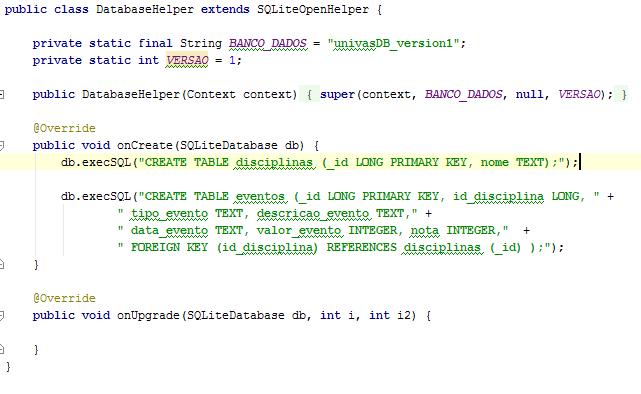
\includegraphics[scale=0.65]{./imagens/2_q_metodologico/4_procedimentos_resultados/42_aplicativo/app4.png}}
		\caption[Método getResults()]{Método \texttt{getResults()}.
		\textbf{Fonte:}Elaborado pelos autores.}
		\label{fig:app4}
	\end{figure}
	
	\pagebreak
	
	\par Foram inseridos mais dois métodos semelhantes ao \texttt{getResults()},
chamados de \texttt{getFouls()} e \texttt{getAgendas()} para recuperar as
faltas e provas agendadas respectivamente. O que diferencia-os é a consulta
SQL, já que no \texttt{getFouls()} foram buscados os dados onde o tipo\_evento
= ‘FALTAS' e no \texttt{getAgendas()} onde o tipo\_evento = 'PROVA\_AGENDADA'.

	\par A fim de estabelecer uma conexão entre o aplicativo e o \textit{web
service} foi preciso conceder a permissão de acesso à internet no arquivo
\texttt{AndroidManifest.xml} da seguinte forma: \texttt{<uses-permission
android:name="android.permission.INTERNET" />}.

	\par Logo após, criou-se uma classe chamada de \texttt{HttpUtil} para ler
informações recebidas do \textit{web service}. Nela foram inseridos dois
métodos, sendo um chamado \texttt{getJsonDisciplinas()} para receber as
informações referentes as disciplinas cursadas e outro denominado
\texttt{getJsonEventos()} para captar os dados de eventos como notas, faltas e
provas agendadas.

	\par Os dois métodos são semelhantes, no entanto, o \texttt{getJsonEventos()}
recebe os dados e transforma-os em objetos da classe \texttt{EventTO} enquanto
o método \texttt{getJsonDisciplinas()} converte os elementos em objetos da
classe \texttt{DisciplineTO}. Na Figura \ref{fig:app5} é possível ver o método
\texttt{getJsonEventos()} incumbido de ler as informações de eventos.

	\begin{figure}[h!] 
		\centerline{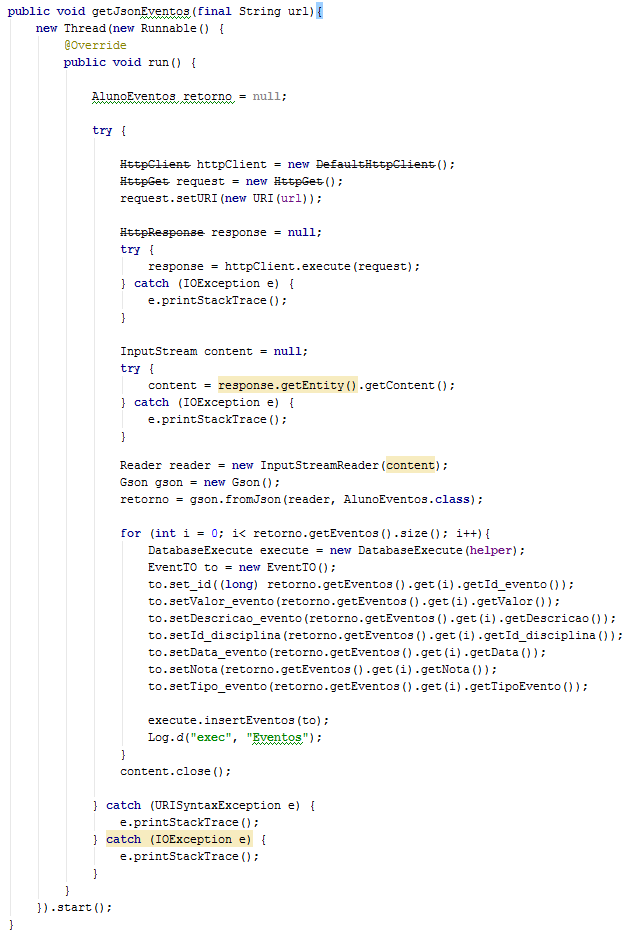
\includegraphics[scale=0.7]{./imagens/2_q_metodologico/4_procedimentos_resultados/42_aplicativo/app5.png}}
		\caption[Método getJsonEventos()]{Método \texttt{getJsonEventos()}.
		\textbf{Fonte:}Elaborado pelos autores.}
		\label{fig:app5}
	\end{figure}
	
	\pagebreak
	
	\par Neste método foi preciso criar uma \textit{thread} separada da
\textit{thread} principal do sistema, evitando travar a aplicação enquanto
recebe as informações vindas do \textit{web service}. Estes dados estão em
formato JSON e foi utilizada a biblioteca Gson para convertê-las para o formato
da classe \texttt{EventTO}. Após a leitura, o objeto da classe \texttt{EventTO}
é enviado para a classe \texttt{DatabaseExecute}, a fim de realizar a inserção
os dados no banco.
	
	\par Para usufruir da biblioteca Gson, foi fundamental adicioná-la como uma
dependência do projeto. Para isso, foi preciso ir ao Menu do Android Studio,
clicando em \textbf{File} e depois em \textbf{Project Structure}. Com a janela
da estrutura do projeto aberta, foi selecionada a aba \textbf{Dependencies} e
depois foi escolhido o ícone de mais (+) para adicionar novas dependências,
conforme mostra a Figura \ref{fig:app6}.
	
	\begin{landscape}
	
		\begin{figure}[h!] 
			\centerline{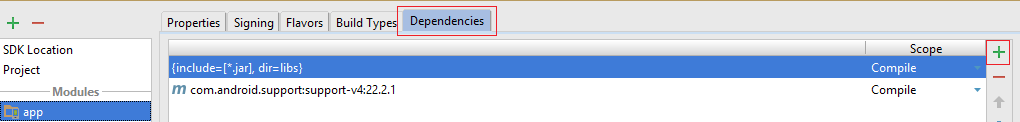
\includegraphics[scale=0.7]{./imagens/2_q_metodologico/4_procedimentos_resultados/42_aplicativo/app6.png}}
			\caption[Adicionando uma dependência ao projeto]{Adicionando uma dependência ao projeto.
			\textbf{Fonte:}Elaborado pelos autores.}
			\label{fig:app6}
		\end{figure}
	
	\pagebreak
	
	\end{landscape}
	
	\par Na tela em que foi aberta localizou-se a biblioteca Gson com o endereço da
Google, logo após selecionou-a e clicou no botão Ok para adicioná-la, como
mostra a Figura \ref{fig:app7}.
	
		\begin{figure}[h!] 
			\centerline{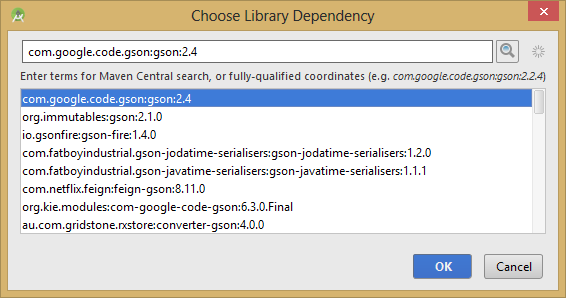
\includegraphics[scale=0.7]{./imagens/2_q_metodologico/4_procedimentos_resultados/42_aplicativo/app7.png}}
			\caption[Adicionando a biblioteca Gson ao projeto]{Adicionando a biblioteca Gson ao projeto.
			\textbf{Fonte:}Elaborado pelos autores.}
			\label{fig:app7}
		\end{figure}
	
	\pagebreak